\documentclass{book}
\usepackage{amsfonts}
\usepackage{amsmath}
\usepackage{graphicx}
\usepackage{epstopdf}
\usepackage{amssymb}
\usepackage{hyperref}
\usepackage{textcomp}
\usepackage{listings}
\usepackage{units}
\usepackage{color}

\definecolor{dkgreen}{rgb}{0,0.6,0}
\definecolor{gray}{rgb}{0.5,0.5,0.5}
\definecolor{mauve}{rgb}{0.58,0,0.82}

\lstset{frame=tb,
  language=Python,
  aboveskip=3mm,
  belowskip=3mm,
  showstringspaces=false,
  columns=flexible,
  basicstyle={\small\ttfamily},
  numbers=none,
  numberstyle=\tiny\color{gray},
  keywordstyle=\color{blue},
  commentstyle=\color{dkgreen},
  stringstyle=\color{mauve},
  breaklines=true,
  breakatwhitespace=true,
  tabsize=3, upquote=true}

\lstMakeShortInline[columns=fixed]|
\setcounter{chapter}{6}

\begin{document}



\chapter[Numerical modeling I]{Numerical modeling of Projectile motion}

There are times when we would like to predict the motion of an object, but we
would like to make a computer do the hard work involved in solving the
equations to get a numeric answer, so we don't have to do it. For example, we
might want to calculate the position of a satellite as it orbits. Or we might
want to calculate the position of the planets as they orbit the Sun. For
simple cases, we might be able to do this by hand, but predicting by hand
where all the planets will be on July 4, 2200 might get tedious without a computer.

As physics students, it is good to know how to approach solving problems on a
computer.\footnote{Most calculators qualify as computers now, since they are
usually programmable. But we are talking about going beyond the built in
functions of calculators or even spreadsheet functions on computers.}

Let's start with some simple problems that we know how to do algebraically so
we can tell if the computer solution is reasonable by comparing to the exact
answer. Then we will tackle things we can't do algebraically.

Consider a ball moving under constant acceleration in one dimension. This is a
kinematics problem. So we can use the kinematic equations you have learned (or
will very shortly learn) in PH121. Let's remind ourselves of what these are: 
\begin{align*}
x  & =x_{o}+v_{o}t+\frac{1}{2}at^{2}\\
v  & =v_{o}+at\\
v^{2}  & =v_{o}^{2}+2a\left(  x-x_{o}\right) \\
x  & =x_{o}+\frac{1}{2}\left(  v_{o}+v\right)  t
\end{align*}
The first equation tells us the position, $x,$ as a function of time. This
could be position in any direction, up and down, or side to side. If it is a
ball being shot into the air, it might be better to write $y$ instead of $x.$
But for now, we will use just $x$ for position in any direction. What this
first equation tells us is that, once the ball is moving, we can find the new
position of the ball by starting with the initial position of the ball,
$x_{o},$ and adding to this initial position how far it has gone in $t$
seconds.
\begin{center}
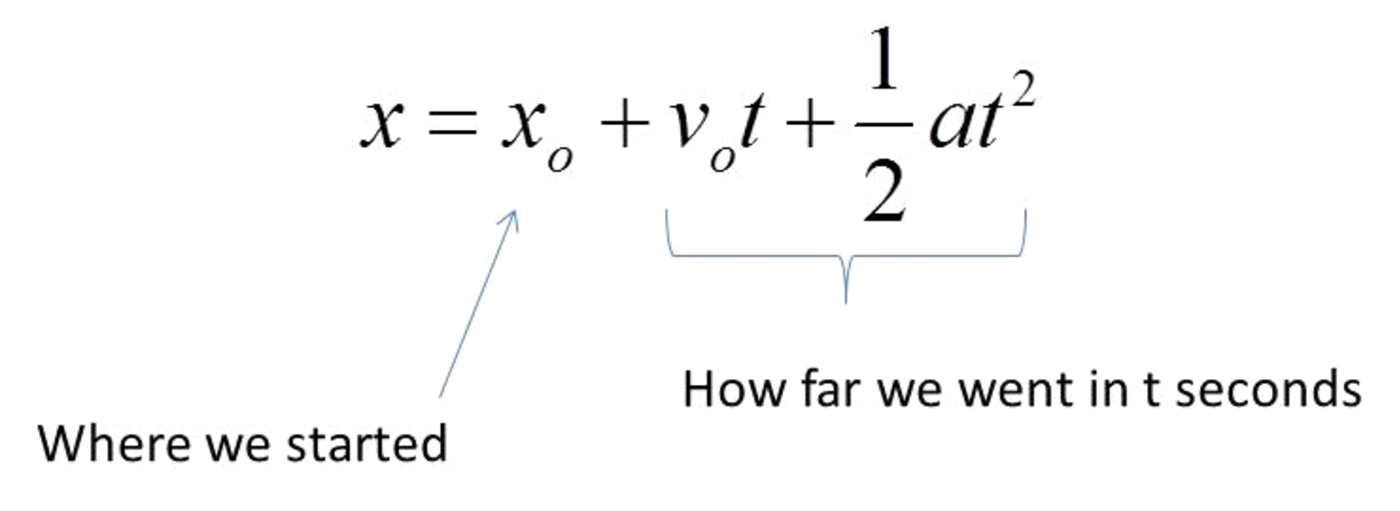
\includegraphics[natheight=1.308300in,natwidth=3.587800in,height=0.9943in,width=2.6911in]{Lab7_figs/kinematicsAnnotated.png} \end{center}
If the ball were going at constant speed, the additional distance would be
just $v_{o}t$. This comes from speed being distance over time.
\begin{align*}
v  & =\frac{d}{t}\\
d  & =vt
\end{align*}
But our ball is accelerating, so we have to add in a little more distance
because our speed is changing. That is what $\frac{1}{2}at^{2}$ does. 


Since the position is a function of $t^{2},$ we know that the position vs.
time graph for our ball will be a parabola.

 
\begin{center}
\fbox{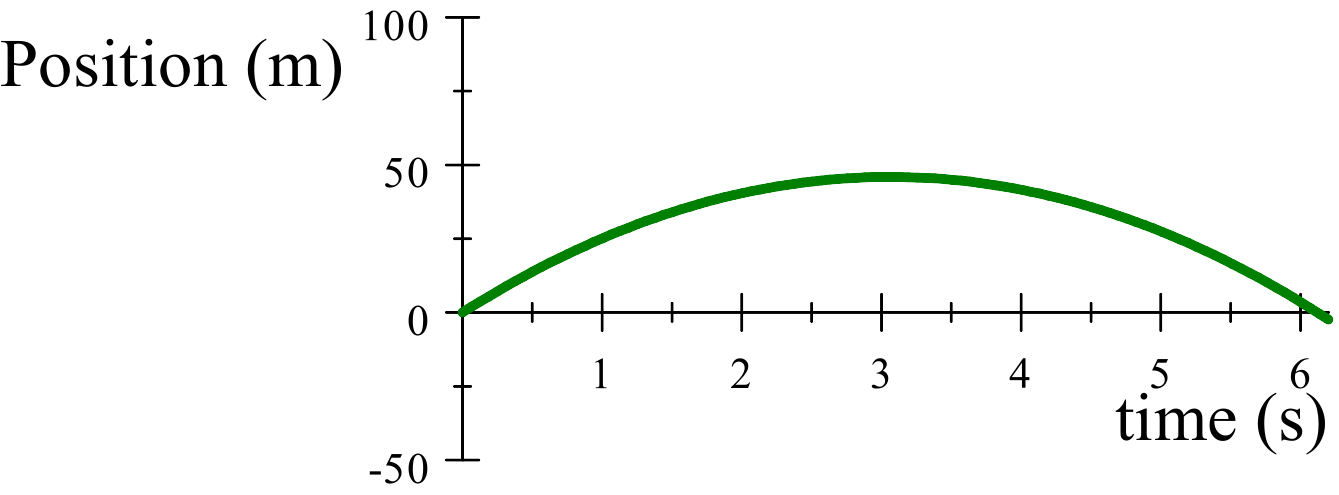
\includegraphics[natheight=1.265200in,natwidth=3.375400in,height=1.2652in,width=3.3754in]{Lab7_figs/PvTSimple.png}}
\end{center}
The second and third equations from our kinematic set give the speed of the
object. The second is the speed as a function of time. Since for this first
problem in programming we will only allow one dimensional motion (at first) we
could say this is the velocity of the object and allow negative values to mean
going the opposite way of positive values. Because the ball is accelerating,
the speed will change. We can see that the velocity changes linearly with
time. Think of a straight line
\[
y=mx+b
\]
our velocity equation is
\[
v=at+v_{o}
\]
on a velocity vs. time graph, this has the form of a straight line. So the
velocity vs. time graph will be a straight line. 
\begin{center}
\fbox{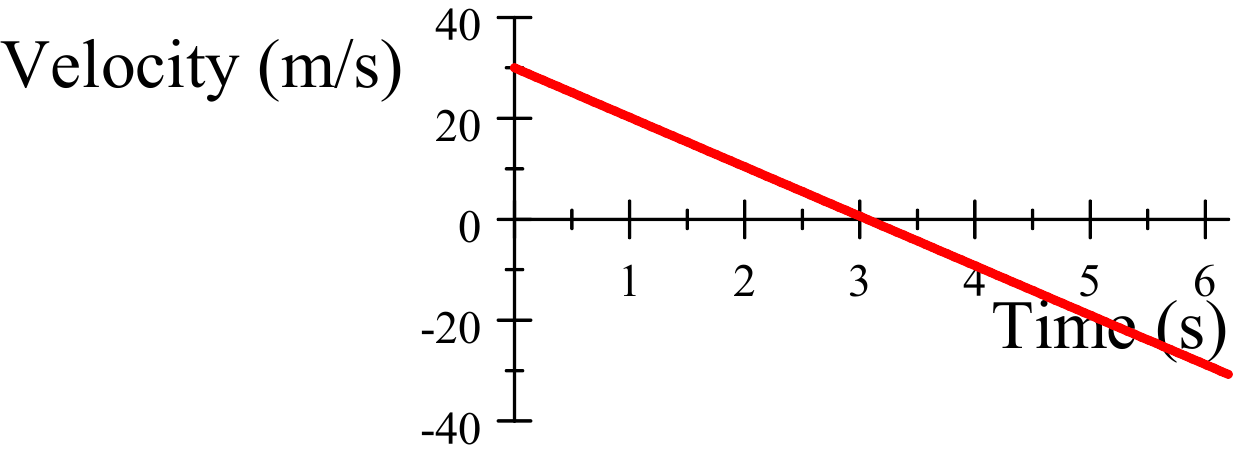
\includegraphics[natheight=1.167500in,natwidth=3.125400in,height=1.1675in,width=3.1254in]{Lab7_figs/VvTSimple.png}}
\end{center}


Our goal is to get the computer to predict this motion. To do this we will use
an idea from calculus\footnote{Not to worry if you are concurrently taking
calculus. We will use very little calculus in this reading, so little that you
probably won't notice it.} that we can take an infinitesimally small amount of
time for our experiment. We will call this very small amount of time a
\textquotedblleft time step\textquotedblright\ and label it $\Delta t.$ Over
this time interval, the change in velocity is essentially zero, that is, over
our very small time interval, we can take $a\approx0,$ then our first
kinematic equation becomes
\[
x_{f}\approx x_{i}+v_{o}\Delta t
\]
Remember that we have only let our experiment run for a very small time,
$\Delta t$, so even if the velocity changed, it would not have changed much.
So our equation will nearly work. In the limit as $\Delta t\rightarrow0$ our
equation will be exact.

Now suppose I want to go an additional small time interval, a second
mini-experiment. That is, I\ let the experiment keep going now starting from
the end of the first mini-experiment from the specific time $t_{1}=\Delta t$
and end this second mini-experiment at the time $t_{2}=t_{1}+\Delta t$ (that
is the second mini-experiment runs from times $\Delta t$ to $2\Delta t$). We
know where the ball is at the end of the first mini-experiment that lasted
$\Delta t$ seconds. But now we let the ball keep falling. Where will it be
after a second $\Delta t$ seconds? We can predict that the next position will
be
\begin{align*}
x(t_{2})  & =x(t_{1})+v(t_{1})\Delta t\\
x(t+\Delta t)  & =x(t_{1})+v(t_{1})\Delta t
\end{align*}
where $x\left(  t_{1}\right)  $ is the position at the end of the first time
interval (our old $x_{f}$). Likewise, $v\left(  t_{1}\right)  $ is the
velocity at the end of the first time interval. At this point, we have to
acknowledge that the speed of the ball is really changing. Otherwise the
ball's position vs. time graph will go in a straight line as shown in the next
figure 
\begin{center}
\fbox{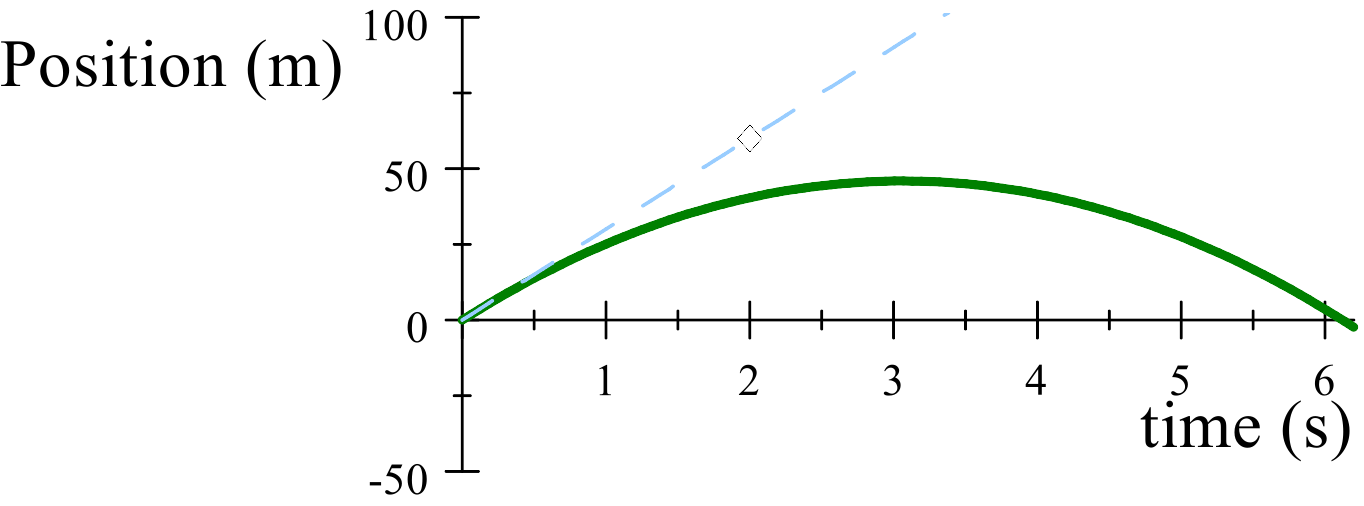
\includegraphics[natheight=1.375000in,natwidth=3.666800in,height=1.375in,width=3.6668in]{Lab7_figs/PvTOnePoint.png}}
\end{center}
The dotted line is what we get when we don't change the velocity. The solid
line is what we should have. But we don't yet know $v\left(  t_{1}\right)  $,
we will have to find it.

We can find $v\left(  t_{1}\right)  $ using the second of our set of kinematic
equations. We can modify the equation
\[
v=v_{o}+at
\]
for the first time interval,
\[
v(t_{1})=v_{o}+a\Delta t
\]
where $v(t_{1})$ means that $v$ is a function of $t$ and we have evaluated $v
$ at $t_{1}.$ This last equation says that at time, $\Delta t,$ the ball is
really going at velocity $v\left(  t_{1}\right)  $ where we have to add (or
subtract, depending on the sign of $a$) the change in velocity due to the
acceleration. That change is velocity is $a\Delta t$ at the end of the first mini-experiment.

At the end of the second mini-experiment the velocity will have changed even
more. I can write this as
\[
v(t+\Delta t)=v(t_{1})+a(t_{1})\Delta t
\]
where again $v(t)$ means that $v$ is a function of $t,$ and $a\left(
t\right)  $ means that $a$ is a function of $t.$In our case, we know the
acceleration is $a\left(  t\right)  =-g,$ and we know that it really does not
depend on time, but let's see how we would find the acceleration if we did not
know this. Let's take Newtons's second law. In one dimension,\footnote{OK,
I\ know it is weird that my $x$-axis is vertical. Usually the vertical axis is
the $y$-axis. But that is just tradition, we can pick our axes any way we
want. And I wanted $x$ to go up and down.}. This may be something you have not
seen yet in PH121, so let me give you Newton's second law. It simply states
that if you add up all the pushes and pulls on an object, the amount of push
or pull left over after opposing pushes cancel is what makes the object change
it's motion. In physics, we call pushes and pulls \textquotedblleft
forces.\textquotedblright\ In a tug-o-war, both sides pull, but they pull in
opposite directions. The winning team has to pull a little bit harder than the
loosing team. This difference in the pull of the two teams is called the net
pull or the net force. That difference in the forces is what makes the rope
accelerate. For our ball, we can write (in calculus notion) \[
\Sigma F_{x}=\frac{d}{dt}\left(  mv\right)  =ma
\]
This means to sum up all the forces in the $x$-direction and it says that that
sum will be equal to the mass of the ball multiplied by the acceleration. If
we know the mass of the ball and the sum of all the pushes and pulls, we can
find the acceleration. If there is no air resistance, all we have is the force
of gravity pulling on our moving ball.
\[
ma=-F_{g}
\]
Then
\[
ma=-mg
\]
or \begin{align*}
a  & =\frac{-mg}{m}\\
& =-g
\end{align*}
So our ball's acceleration is just the acceleration due to gravity.
\[
a\left(  t\right)  =-g
\]
which is not time dependent. This is not very surprising. But what is
important here is the method for obtaining the acceleration, and this method
is general---we can use it in more complicated situations. We will do this
each time we need to find an acceleration for our systems.\footnote{For those
who are taking PH 121 this semester, have a more experienced student work with
you on this part until your PH121 class catches up to net force.}

For our falling ball, then, we could write our second kinematic equation as
\[
v(t+\Delta t)=v(t_{1})-g\Delta t
\]
But note that in our computer formulation, we did not have to assume the
acceleration was constant. In our problem the acceleration \emph{is} constant,
but in the problems to follow, it will not be! Our method can handle
non-constant acceleration. That is more than the kinematic equations can do.
This is exciting!

At this point we have two equations that calculate a new position and velocity
forward in time, based on what the ball's position and speed currently are: \begin{align*}
x(t_{2})  & =x(t+\Delta t)=x(t_{1})+v(t_{1})\Delta t\\
v(t_{2})  & =v(t+\Delta t)=v(t+\Delta t)=v(t_{1})+a(t_{1})g\Delta t
\end{align*}
So far we have only talked about calculating two positions (two
mini-experiments), but we can use these equations to get a general expression
for the next position, and the next, and the next to as many mini-experiments
as we want.
\begin{align*}
x(t+\Delta t)  & =x(t)+v(t)\Delta t\\
v(t+\Delta t)  & =v(t)+a(t)g\Delta t
\end{align*}
These mean to take the position at the current time, $x(t),$ and add the
current speed, $v\left(  t\right)  $ times $\Delta t$ to get the next $x$
position $x\left(  t+\Delta t\right)  .$ And also take the speed at the
current time, $v(t),$ and add the current acceleration, $a\left(  t\right)  $
times $\Delta t$ to get the next speed$,$ $v\left(  t+\Delta t\right)  .$ By
doing this, over and over we can find the position of the ball at each time
for a whole ball flight.

You will notice that these expressions are coupled: the new position depends
on the previous velocity, and the new velocity depends on the previous
position. We have to use the equations together. To find the solution we will
take a small step in time, $\Delta t,$ and calculate a new position. We will
also calculate a new speed. Then we will use the new speed to find a new new
position an additional $\Delta t$ later, and the new new position to find a
new new speed. We step these two quantities forward in time one $\Delta t$ at
a time. We can repeat the process indefinitely.

Let's try an example. Suppose we throw a ball straight up with an initial
velocity of $v_{o}=30 \operatorname{m} / \operatorname{s} $ and an initial position of $x_{o}=0$ (measured vertically) at $t_{0}=0 \operatorname{s} .$ Let's take time steps of size $\Delta t=0.001 \operatorname{s} .$ We can calculate the next position at $t_{1}=\Delta t$ 
\begin{align*}
x(t_{1})  & =x(t_{0})+v(t_{0})\Delta t\\
x(t_{1})  & =0+30\frac{ \operatorname{m} }{ \operatorname{s} }\times0.001 \operatorname{s} \\
& =0.03 \operatorname{m} \end{align*}
our ball has moved to up to the position $x=0.03 \operatorname{m} .$ Our ball will have changed speed. We can find the new speed as
\begin{align*}
v(t_{1})  & =v(t_{0})+a(t)\Delta t\\
v(t_{1})  & =30\frac{ \operatorname{m} }{ \operatorname{s} }-9.8\frac{ \operatorname{m} }{ \operatorname{s} ^{2}}\times0.001 \operatorname{s} \\
& =29.\,\allowbreak99\frac{ \operatorname{m} }{ \operatorname{s} } \end{align*}
as we would expect, the ball has slowed down a little. In the next time
interval, $t_{2}=t_{1}+\Delta t$, the ball will move to the new position
\begin{align*}
x(t_{2})  & =x(t_{1})+v(t_{1})\Delta t\\
x(t_{2})  & =0.03 \operatorname{m} +29.\,\allowbreak99\frac{ \operatorname{m} }{ \operatorname{s} }\times0.001 \operatorname{s} \\
& =0.059\,99 \operatorname{m} \end{align*}
Notice that we used the new velocity at $t_{1}$ to find this second position
at $t_{2}$. We need to find a new velocity at this position
\begin{align*}
v(t_{2})  & =v(t_{1})+a(t_{1})\Delta t\\
v(t_{2})  & =29.\,\allowbreak99\frac{ \operatorname{m} }{ \operatorname{s} }-9.8\frac{ \operatorname{m} }{ \operatorname{s} ^{2}}\times0.001 \operatorname{s} \\
& =29.\,\allowbreak98\frac{ \operatorname{m} }{ \operatorname{s} } \end{align*}
We can use this to find the third position 
\begin{align*}
x(t_{3})  & =x(t_{2})+v(t_{2})\Delta t\\
x(t_{3})  & =0.059\,99 \operatorname{m} +29.\,\allowbreak98\frac{ \operatorname{m} }{ \operatorname{s} }\times0.001 \operatorname{s} \\
& =0.089\,97 \operatorname{m} \end{align*}
and the velocity at this position \begin{align*}
v(t_{3})  & =v(t_{2})+a(t_{2})\Delta t\\
v(t_{3})  & =29.\,\allowbreak98\frac{ \operatorname{m} }{ \operatorname{s} }-9.8\frac{ \operatorname{m} }{ \operatorname{s} ^{2}}\times0.001 \operatorname{s} \\
& =29.\,\allowbreak97\frac{ \operatorname{m} }{ \operatorname{s} } \end{align*}


We can keep marching along, one $\Delta t$ at a time finding new positions,
then finding new speeds, then using the new speed to find a new position, and
finding the new position to find a new speed, and the new speed to find a new
position, etc.

There is a typical short hand for these equations \begin{align*}
x_{n+1}  & =x_{n}+v_{n}\Delta t\\
v_{n+1}  & =v_{n}-g\Delta t
\end{align*}
What this means is that we have labeled each new $x$ and $v$ by how many time
steps, $\Delta t$, we have taken. The first $\Delta t$ will be $n=1,$ the
second $n=2,$ and so on. Just to be clear, let's compare \begin{align*}
x(t+\Delta t)  & =x(t)+v(t)\Delta t\\
x_{n+1}  & =x_{n}+v_{n}\Delta t
\end{align*}
This means that we start with the initial velocity, $v_{0}$ at the initial
position $x_{0}.$ We use these to calculate the position $x_{1}$ and the speed
$v_{1}$ a time $t=\Delta t$ later.
\begin{align*}
x_{1}  & =x_{0}+v_{0}\Delta t\\
v_{1}  & =v_{0}-g\Delta t
\end{align*}
Then we start over with the new initial velocity, $v_{1}$ at the initial new
position $x_{1}$ and use them to calculate the position $x_{2}$ and the speed
$v_{2}$ an additional time $\Delta t$ later ($t=2\Delta t$).
\begin{align*}
x_{2}  & =x_{1}+v_{1}\Delta t\\
v_{2}  & =v_{1}-g\Delta t
\end{align*}
Then we use $x_{2}$ and $v_{2}$ to find $x_{3}$ and $v_{3}$
\begin{align*}
x_{3}  & =x_{2}+v_{2}\Delta t\\
v_{3}  & =v_{2}-g\Delta t
\end{align*}
and so forth. Here is what we get after many iterations:


\begin{center}
\fbox{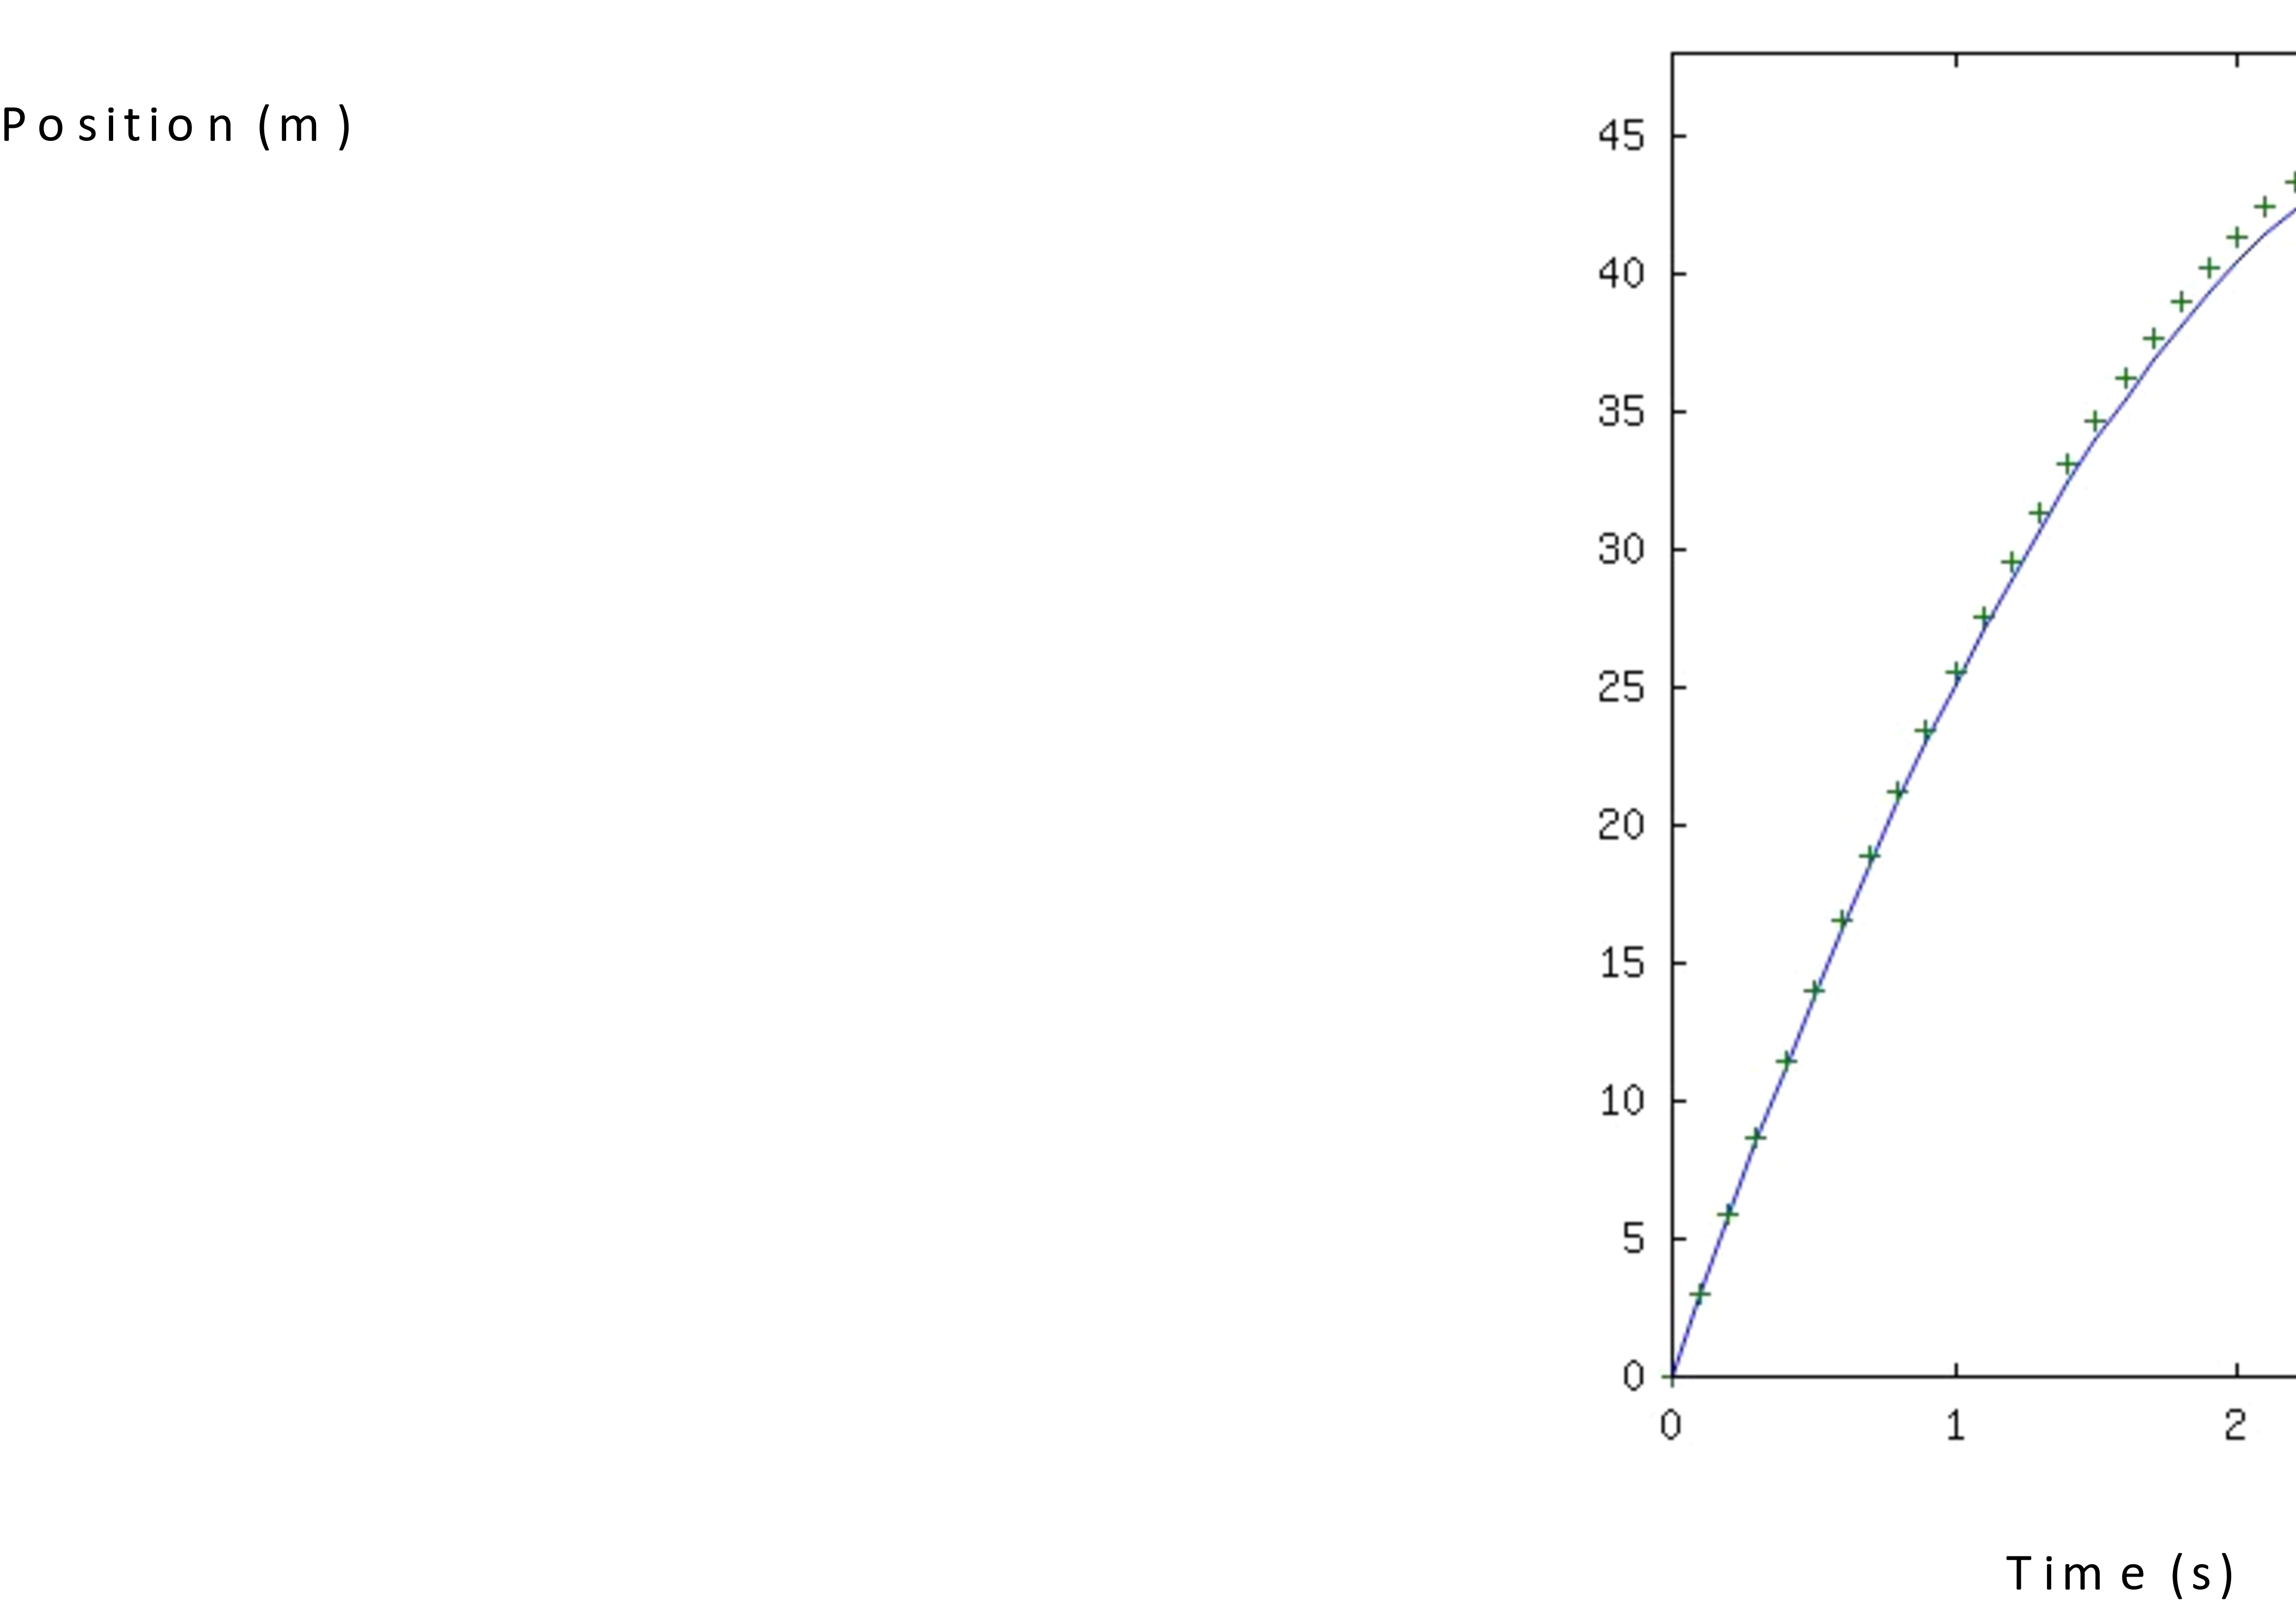
\includegraphics[natheight=7.383800in,natwidth=10.552400in,height=1.708in,width=2.4362in]{Lab7_figs/MLQ2XV07.png} }

\end{center}
the solid line is the result of the kinematic equation (the correct result).
The little plus signs are our computer solution. It is not too bad, but it is
not too good either. Of course, if we let our $\Delta t$ get smaller, we will
have a better solution.

 
\begin{center}
\fbox{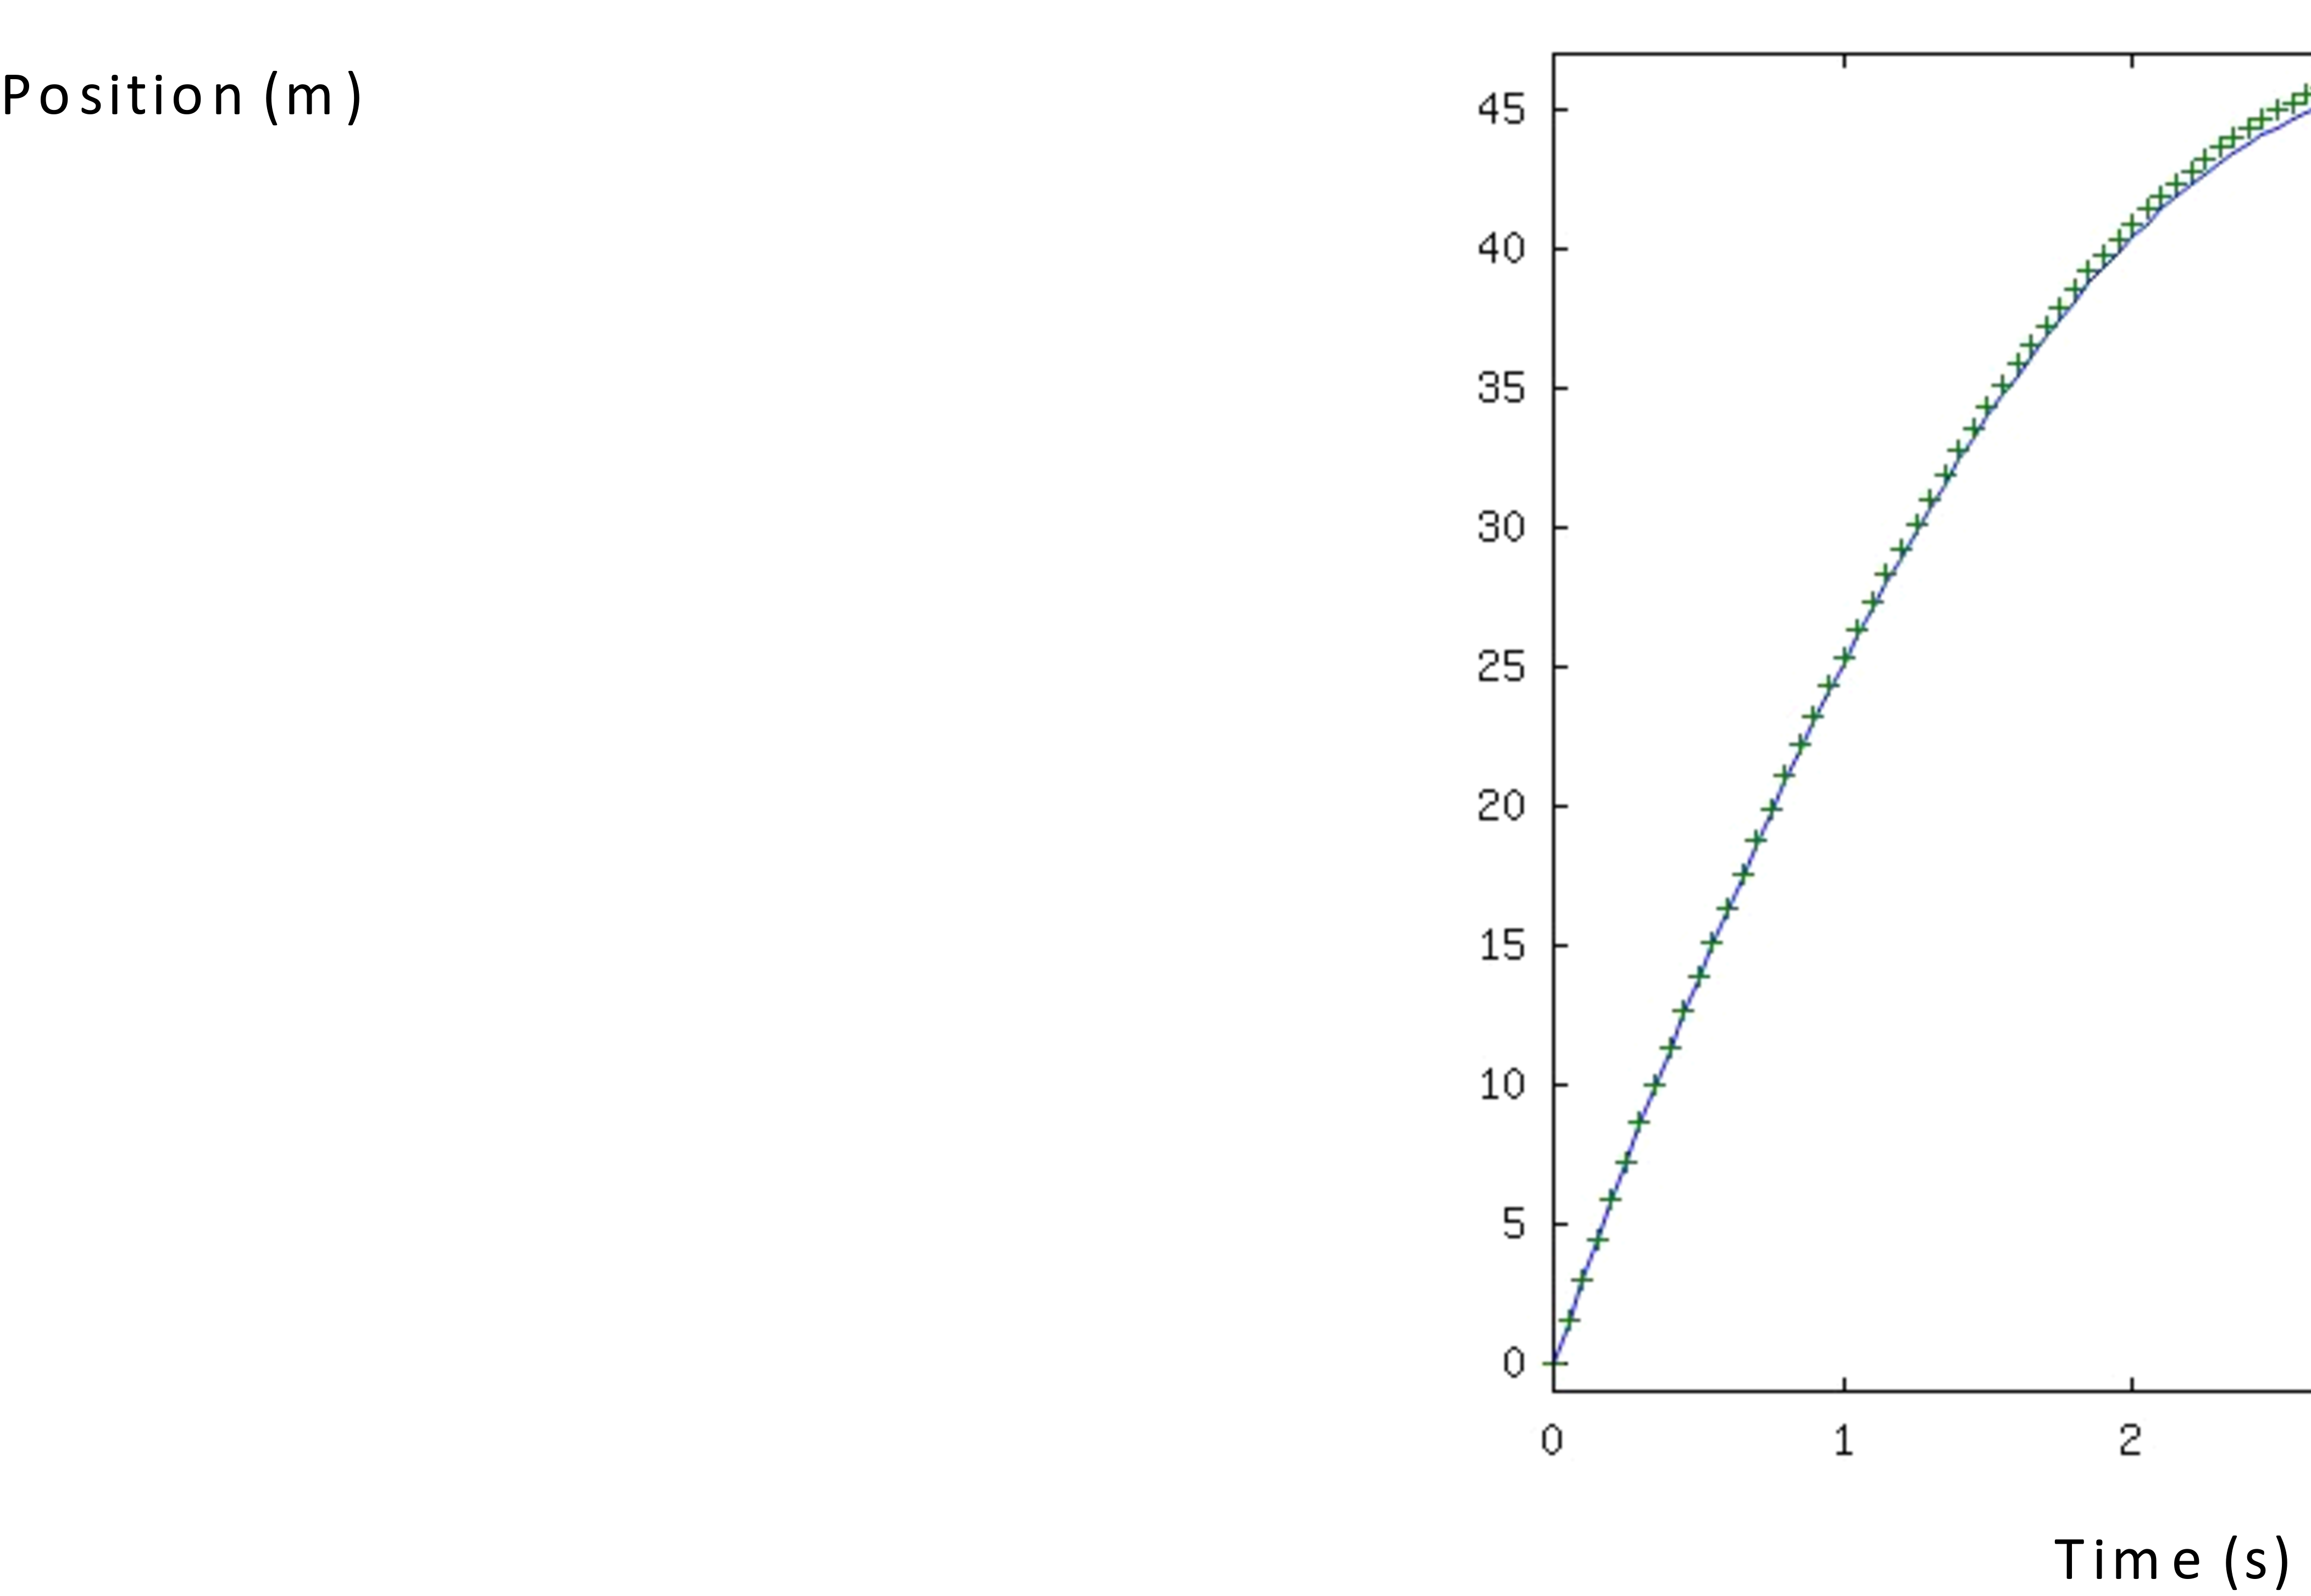
\includegraphics[natheight=7.258400in,natwidth=10.510100in,height=1.6994in,width=2.4543in]{Lab7_figs/MLQ2XV08.png} }
\end{center}
Notice that there are many more small plus signs now. We had to do more
calculations to get the improvement. This is the cost of the smaller $\Delta
t.$ If we let $\Delta t$ be very small the curves lie right on top of each other.

 
\begin{center}
\fbox{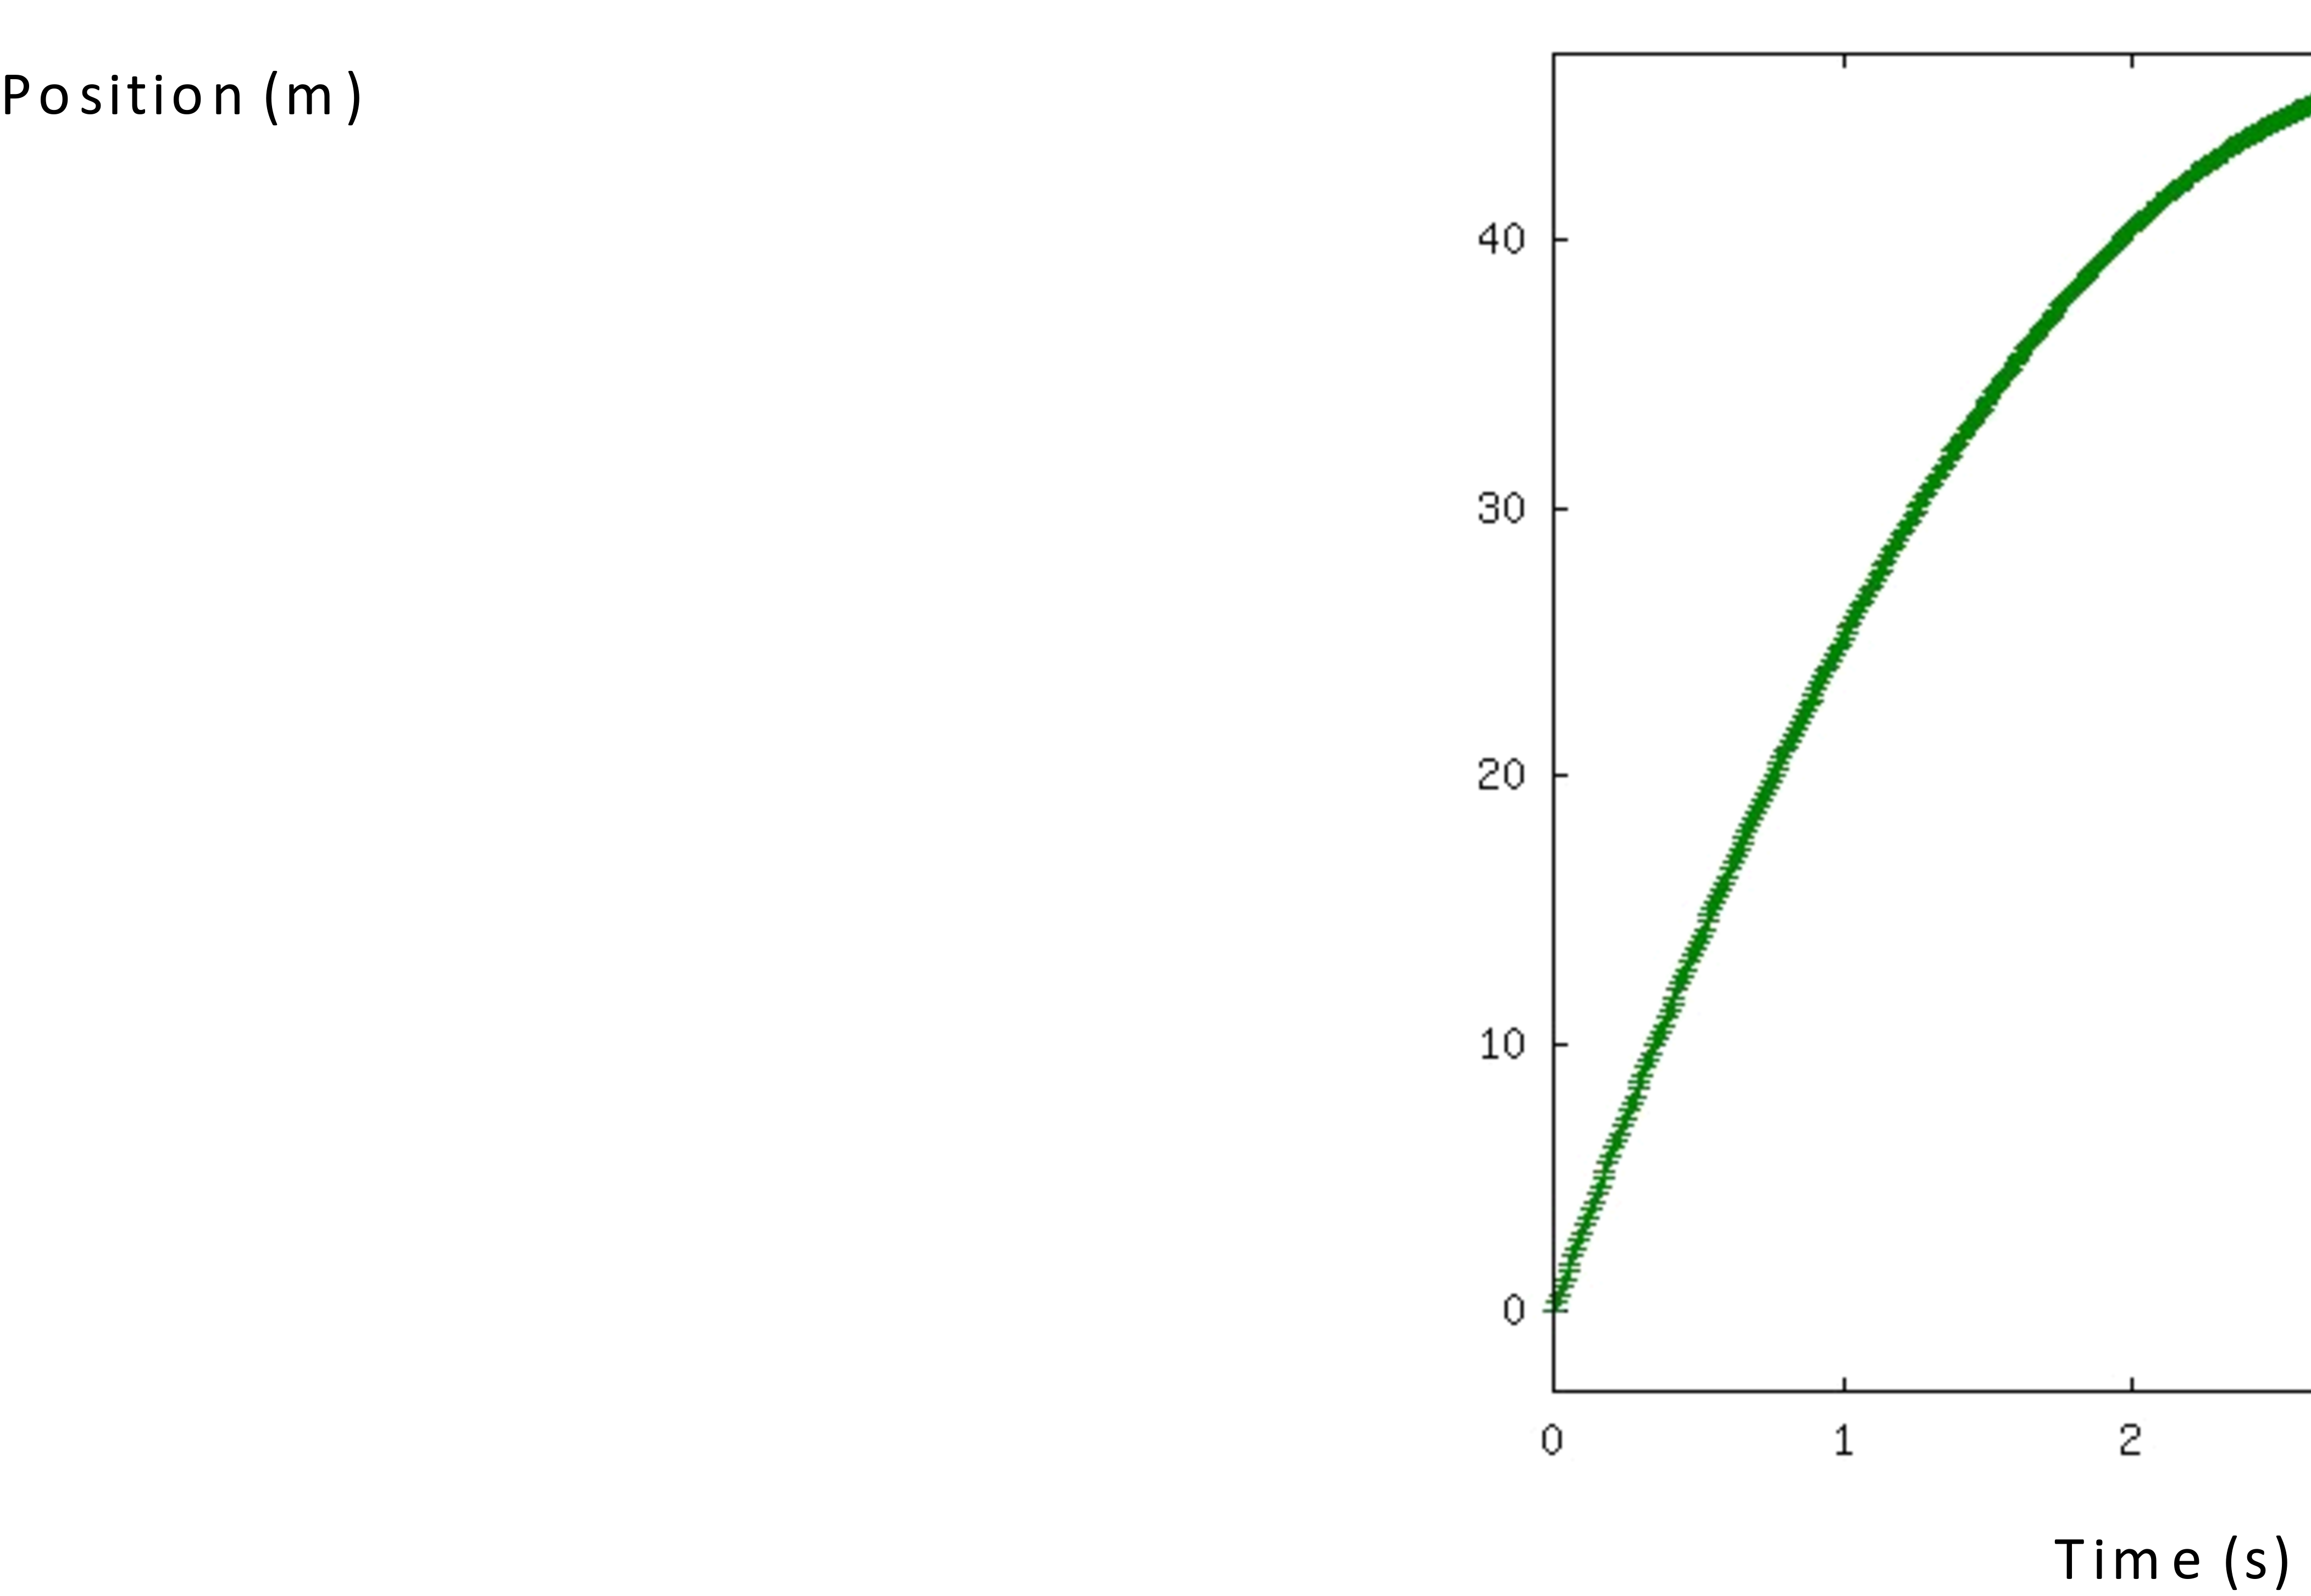
\includegraphics[natheight=7.258400in,natwidth=10.510100in,height=1.5169in,width=2.1897in]{Lab7_figs/MLQ2XV09.png}}
\end{center}
Euler came up with this method back in the 1700's and we still call this
method of numerically finding results \emph{Euler's method} (pronounced
like\textquotedblleft oiler\textquotedblright).

Let's take a moment and see what went wrong when $\Delta t$ was not small enough.

 
\begin{center}
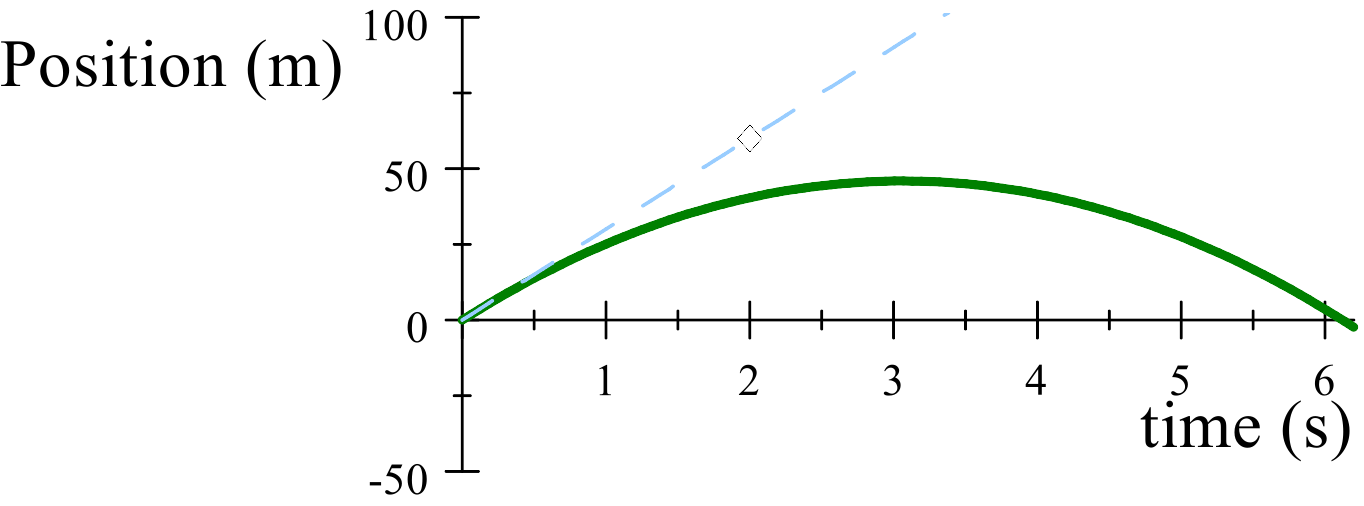
\includegraphics[natheight=1.289400in,natwidth=3.437600in,height=1.2894in,width=3.4376in]{Lab7_figs/PvTOnePoint.png}
\end{center}
In the figure, we can see a solid curve (green if you are seeing this in
color). Let's suppose the solid curve represents the actual position of the
ball as a function of time. Lets also suppose $\Delta t=2 \operatorname{s} .$ If we use the method we have described to find the position as a function
of time, we will get an $x_{1}$ that is shown as a diamond on the graph. We
have
\begin{align*}
x_{1}  & =x_{0}+v_{0}\Delta t\\
v_{1}  & =v_{0}-g\Delta t
\end{align*}
if we let $v_{o}=30 \operatorname{m} / \operatorname{s} $ and $x_{o}=0$ like before, we get
\begin{align*}
x_{1}  & =0+30\frac{ \operatorname{m} }{ \operatorname{s} }\times2 \operatorname{s} =60 \operatorname{m} \\
v_{1}  & =30\frac{ \operatorname{m} }{ \operatorname{s} }-9.81\frac{ \operatorname{m} }{ \operatorname{s} ^{2}}\times2 \operatorname{s} =\allowbreak10.\,\allowbreak38\frac{ \operatorname{m} }{ \operatorname{s} } \end{align*}
This is much too high. That is because our method assumes \[
\frac{dx}{dt}=v_{o}
\]
for this entire time step. But observing the solid curve shows us that $dx/dt
$ is not constant along the path. The slope changes because there is a
negative acceleration. So we have over-estimated $x_{1}.$ This error will
compound as we go. For the next $\Delta t$ we start with $x_{1}$ and our new
slope $v_{1}$ and try to find $x_{2}.$
\begin{align*}
x_{2}  & =x_{1}+v_{1}\Delta t\\
v_{2}  & =v_{1}-g\Delta t
\end{align*}
or, given our initial conditions, \begin{align*}
x_{2}  & =60 \operatorname{m} +\allowbreak10.\,\allowbreak38\frac{ \operatorname{m} }{ \operatorname{s} }\times2 \operatorname{s} =\allowbreak80.\,\allowbreak76 \operatorname{m} \\
v_{2}  & =\allowbreak10.\,\allowbreak38\frac{ \operatorname{m} }{ \operatorname{s} }-9.81\frac{ \operatorname{m} }{ \operatorname{s} ^{2}}\times2 \operatorname{s} =\allowbreak-9.\,\allowbreak24\frac{ \operatorname{m} }{ \operatorname{s} } \end{align*} \begin{center}
\fbox{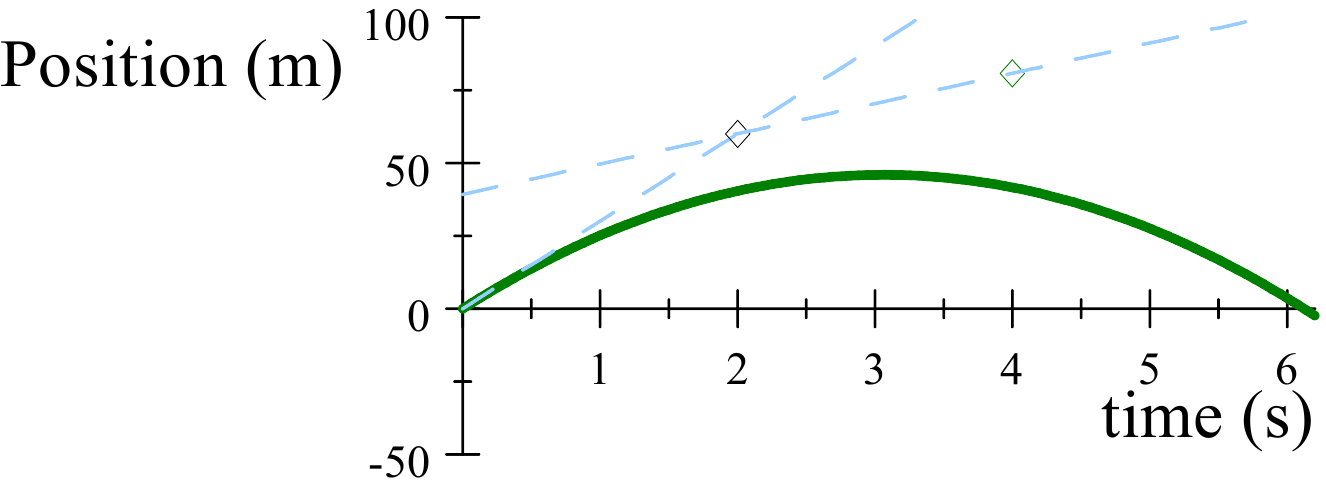
\includegraphics[natheight=1.252200in,natwidth=3.339900in,height=1.2522in,width=3.3399in]{Lab7_figs/PvTTwoPoints.png} }
\end{center}


We can see that if $\Delta t$ is too big, we take a step that is too high
because our slope is too big. This continually happens at each step. Our
solution gets poorer and poorer.

We can see that using numerical techniques requires some caution. The farther
from your initial conditions you get, the poorer the result will be. In other
words, if I\ look at $t=0.5$ seconds, the soliton is not too bad. But at $t=4$
seconds our solution was $\allowbreak39.\,\allowbreak163 \operatorname{m} $ off.

You might be tempted to ask \textquotedblleft then why do
this?\textquotedblright\ The answer is, we often do not have easy kinematic
equations that will solve our problems. Suppose, for example, the acceleration
is not constant.

\section{Euler and Simple Systems with Not-So-Simple Dynamics.}

Suppose we throw a ball, but we have air resistance. Your PH121 class only has
you throw balls in a vacuum--something that is only fun if you have a space
suit. Real balls have air resistance. To model air resistance is really a
PH123 problem. So I will just give you a formula for the force due to air
resistance here. There is a resistive force
\[
F_{R}=\frac{1}{2}D\rho Av^{2}
\]
that depends on the cross-sectional area of the ball, $A,$ the density of the
air, $\rho,$ the speed of the ball, $v,$ and the ball's drag coefficient, $D,$
that contains the effects like surface ruffness and shape of the ball. So we
have two forces working on the ball now, the force due to gravity, and the
resistive force. If we throw the ball straight up, then we only have forces in
one dimension. We can use our Newton's second law method to find the acceleration! 
\[
\Sigma F_{x}=ma=-F_{g}+F_{R}
\]
so \[
a=\frac{-F_{g}+F_{R}}{m}
\]
or \begin{align*}
a  & =\frac{-mg+\frac{1}{2}D\rho Av^{2}}{m}\\
& =-g+\frac{D\rho Av^{2}}{2m} \end{align*}


Notice that this acceleration changes when $v$ changes. And we know that $v$
does change as the ball goes up. We can't use the kinematic equations at all
with a changing acceleration. But we can use our Euler method. \begin{align*}
x(t+\Delta t)  & =x(t)+v(t)\Delta t\\
v(t+\Delta t)  & =v(t)+a\left(  t\right)  \Delta t
\end{align*}
or \begin{align*}
x_{n+1}  & =x_{n}+v_{n}\Delta t\\
v_{n+1}  & =v_{n}+a_{n}\Delta t
\end{align*}
The only difference is that now our acceleration is not $-g,$ but
$a=-g+\frac{D\rho Av^{2}}{2m}.$ So instead of
\begin{align*}
x_{n+1}  & =x_{n}+v_{n}\Delta t\\
v_{n+1}  & =v_{n}-g\Delta t
\end{align*}
we will have \begin{align*}
x_{n+1}  & =x_{n}+v_{n}\Delta t\\
v_{n+1}  & =v_{n}+\left(  -g+\frac{D\rho A\left(  v(t)\right)  ^{2}} {2m}\right)  \Delta t
\end{align*}


The rest of the method stays the same. In fact, to change physical systems we
usually only need to change the acceleration function. This implies that we
could build a general Euler solver, and then just modify the acceleration
part. That is such a good idea that there are standard notations for this.

\section{Standard Euler Notation}

This is not really needed for our lab today, but might be helpful if you have
to write a Euler code in the future. It is convenient if you are a computer
programer (which you now are!) to write this method more generally, in
particular, if we have two coupled differential equations of the
form\footnote{In computer programming books and Numerical Methods Books, they
usually switch the $v$ to the letter $y$ to be more general. That is because
you may want to solve a differential equation that is not in terms of position
vs time. But for this first view of Euler's method, I\ will stick with $v.$}
\begin{align*}
\frac{dx}{dt}  & =v\left(  t\right)  =f(x,v,t)\\
\frac{dv}{dt}  & =a\left(  t\right)  =g(x,v,t)
\end{align*}
All we have done is to write the speed as $f(x,v,t)$ and the acceleration as
$g(x,v,t).$ Then we step them forward in time according to \begin{align*}
x_{n+1}  & =x_{n}+f(x_{n},v_{n},t_{n})\Delta t\\
v_{n+1}  & =v_{n}+g(x_{n},v_{n},t_{n})\Delta t
\end{align*}
where the subscript $n$ refers to the number of time steps we have taken, and
$t_{n}$ refers to the time of the $n^{\text{th}}$ time step. This is really
nothing new for us. We just wrote $a$ and $v$ a different way.
\begin{align*}
f(x,v,t)  & =v\left(  t\right) \\
g(x,v,t)  & =a\left(  t\right)
\end{align*}
so we have only invented a more difficult way to write our equations. We are
right back to
\begin{align*}
x_{n+1}  & =x_{n}+v_{n}\Delta t\\
v_{n+1}  & =v_{n}+a_{n}\Delta t
\end{align*}
But if I have more than two coupled equations (say, we let the ball move in
two dimensions), the extension is quite straightforward to incorporate the
additional equations in the new notation. If
\begin{align*}
\frac{dx}{dt}  & =f_{x}(x,y,v_{x,}v_{y},t)\\
\frac{dy}{dt}  & =f_{y}(x,y,v_{x,}v_{y},t)
\end{align*} \begin{align*}
\frac{dv_{x}}{dt}  & =g_{x}(x,y,v_{x,}v_{y},t)\\
\frac{dv_{y}}{dt}  & =g_{y}(x,y,v_{x,}v_{y},t)
\end{align*}
then the Euler method notation would dictate
\begin{align*}
x_{n+1}  & =x_{n}+f_{x}(x_{n},y_{n},v_{x_{n},}v_{y_{n}},t_{n})(\Delta t)\\
y_{n+1}  & =y_{n}+f_{y}(x_{n},y_{n},v_{x_{n},}v_{y_{n}},t_{n})(\Delta t)\\
v_{x_{n+1}}  & =v_{x_{n+1}}+g_{x}(x_{n},y_{n},v_{x_{n},}v_{y_{n}} ,t_{n})(\Delta t)\\
v_{y_{n+1}}  & =v_{y_{n+1}}+g_{y}(x_{n},y_{n},v_{x_{n},}v_{y_{n}} ,t_{n})(\Delta t)
\end{align*}


Let's see what our ball with air resistance would look like in this notation. \begin{align*}
x_{n+1}  & =x_{n}+f(x_{n},y_{n},v_{x_{n},}v_{y_{n}},t_{n})(\Delta t)\\
v_{n+1}  & =v_{n}+g(x_{n},y_{n},v_{x_{n},}v_{y_{n}},t_{n})(\Delta t)
\end{align*}
with
\begin{align*}
f(x_{n},y_{n},v_{x_{n},}v_{y_{n}},t_{n})  & =v\left(  t_{n}\right) \\
g(x_{n},y_{n},v_{x_{n},}v_{y_{n}},t_{n})  & =-g+\frac{D\rho Av_{n}(t_{n})^{2} }{2m} \end{align*}
We really just write out the acceleration equation on a different line, and
that makes the code easier to write.

In the event that your time steps are infinitely small (i.e. $\Delta
t\rightarrow0$), the Euler method will give you an exact solution. In reality,
we cannot take infinitely small time steps. We can imagine making them really,
really small, but then we have to take many, many calculations. For example,
if my time step were as small as $1 \operatorname{ns} $, I would have to take one billion steps forward in time just to cover one
second of experimental time!

The issue of taking large number of steps is not the only problem we face.
Only infinitely small time steps will give you an exact solution. Any time
step that is not infinitely small will only give you an approximate solution.
The larger the time step, the less accurate the approximation. It turns out
that these approximate solutions turn sour quickly, as we will see when we
tackle mass-spring systems. Even with a very small time step, an Euler's
method simulation of the mass-spring system becomes unphysical after just one
or two oscillations!

So we should ask, is this really useful? Is there some way to make numerical
modeling more accurate? The answer, of course, is yes to both questions.

\section{Beyond Euler: The Runge-Kutta Method.}

We won't go beyond the Euler method in this class, unless you want to try for
the extra credit. But it is useful to think of how we would. So read this next
part, but look fop the concepts of how to make Euler better, and don't worry
about the details of writing computer code to make the improvement happen.

The nastiness that evolves from the Euler method boils down to one simple
fact: we assume that the rate of change of the variable is constant over a
given time step. Obviously, this assumption is wrong in practically every
circumstance\footnote{The only exception would be, for example, where velocity
was constant. In this case a numerical solution would be completely
unwarranted.}. To make matters even worse, we take our \textquotedblleft
constant\textquotedblright\ rate of change from the endpoint of the time
interval, and the rate of change at the endpoint is by no means representative
of the entire interval. Here is an example. In the figure below, the solid
curve is the function we are trying to find. We will start at $t=10 \operatorname{s} .$ \begin{center}
\fbox{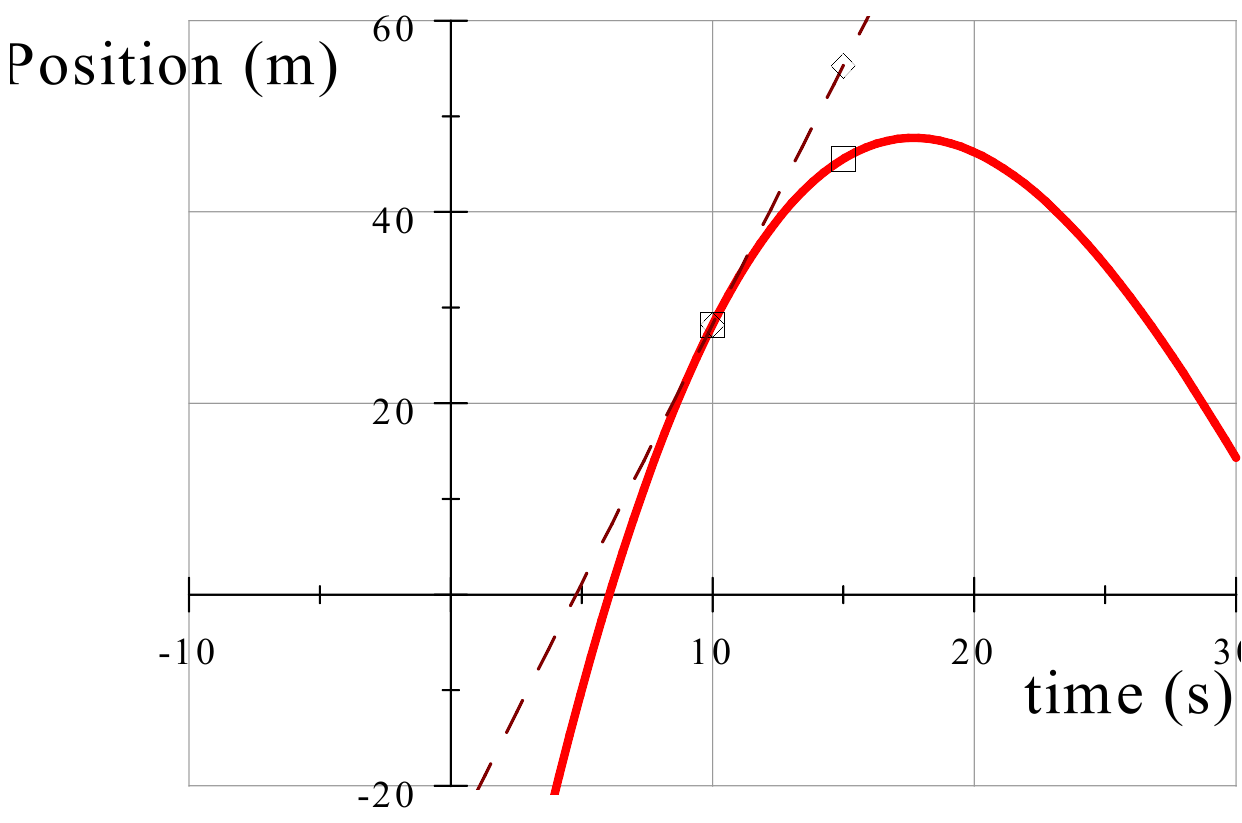
\includegraphics[natheight=2.085900in,natwidth=3.128900in,height=2.0859in,width=3.1289in]{Lab7_figs/ParabTan.png} }
\end{center}
I want to use a time step of $\Delta t=5 \operatorname{s} $ (way to large). We see that our Euler's method starts with our initial time
at $t=10 \operatorname{s} $ and makes a step
\[
x_{1}=x_{0}+v_{0}\Delta t
\]
that is on the straight line. The slope of the straight line is given by
$v_{0.}=\frac{dx}{dt}$ right at our starting point, $(x_{o},10 \operatorname{s} ).$ We get the position $x_{1}$ marked by the small diamond. But, as we
expect, this is not on the true curve at all!

An obvious improvement would be made if we could somehow estimate what the
average value of the slope (derivative) over the time interval would be. It
would logically be better to use this average value while progressing a given
variable over time (for example, using the average velocity over a time
interval while evaluating the position).
\begin{center}
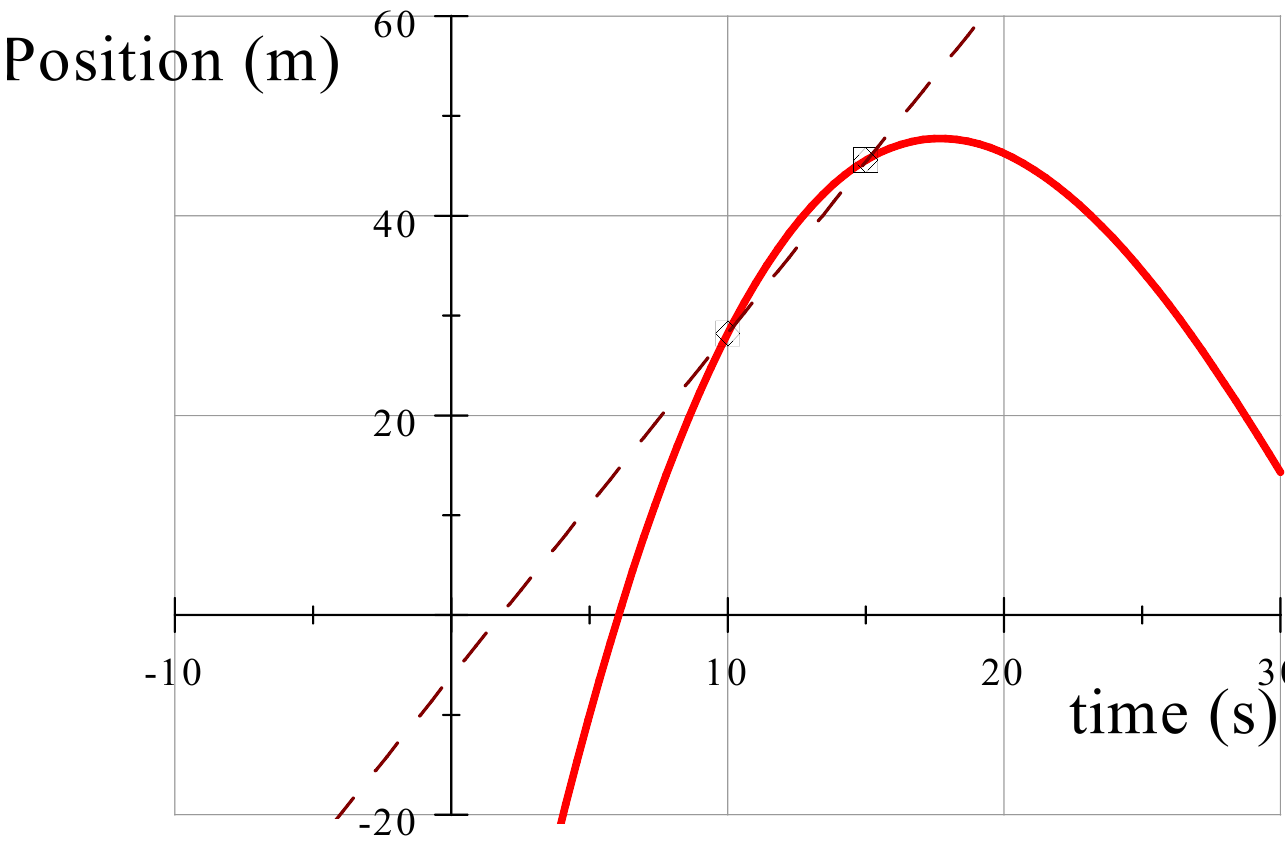
\includegraphics[natheight=2.159400in,natwidth=3.239600in,height=2.1594in,width=3.2396in]{Lab7_figs/Parab2Points.png}
\end{center}
This is quite an improvement as you can see.

There are methods for doing just this. One way is to take a trial step across
the entire interval, estimate the values of the derivatives at the midpoint of
the interval, and then use the midpoint derivatives to step over the entire
interval. For the set of coupled differential equations from before,
\begin{align*}
\frac{dx}{dt}  & =f(x,v,t)\\
\frac{dv}{dt}  & =g(x,v,t)
\end{align*}
this process is reflected by numerical iterations of the form
\begin{align*}
k_{x1}  & =(\Delta t)f(x_{n},v_{n},t_{n})\\
k_{y1}  & =(\Delta t)g(x_{n},v_{n},t_{n})\\
k_{x2}  & =(\Delta t)f\left(  x_{n}+\frac{k_{x1}}{2},v_{n}+\frac{k_{v1}} {2},t_{n}+\frac{\Delta t}{2}\right) \\
k_{y2}  & =(\Delta t)g\left(  x_{n}+\frac{k_{x1}}{2},v_{n}+\frac{k_{v1}} {2},t_{n}+\frac{\Delta t}{2}\right) \\
x_{n+1}  & =x_{n}+k_{x2}\\
v_{n+1}  & =y_{n}+k_{v2} 
\end{align*}
Lets take this apart to see what it means

The last two equations project our position and another variable (for us
velocity) forward to the next position. 
\begin{align*}
x_{n+1}  & =x_{n}+k_{x2}\\
v_{n+1}  & =v_{n}+k_{v2} \end{align*}


If we were using Euler's method we would know what these look like from our
previous work: 
\begin{align*}
x_{n+1}  & =x_{n}+v_{n}\Delta t\\
v_{n+1}  & =v_{n}+a_{n}\Delta t
\end{align*}
We could identify \begin{align*}
k_{x2}  & =v_{n}\Delta t\\
k_{v2}  & =a_{n}\Delta t
\end{align*}
or we could write these as
\begin{align*}
k_{x2}  & =(\Delta t)f(x_{n},v_{n},t_{n})\\
k_{v2}  & =(\Delta t)g(x_{n},v_{n},t_{n})
\end{align*}
because
\begin{align*}
f(x_{n},v_{n},t_{n})  & =v_{n}\\
g(x_{n},v_{n},t_{n})  & =a_{n}=-g
\end{align*}
This would just be a more obscure way to write Euler's method. We would use
the derivative or slope at $x_{1}$ to find $x_{2}.$ But we want to find an
average slope over the interval $x_{1}$ to $x_{2}.$ To do this we start with
the Euler steps
\begin{align*}
k_{x1}  & =(\Delta t)f(x_{n},v_{n},t_{n})\\
k_{v1}  & =(\Delta t)g(x_{n},v_{n},t_{n})
\end{align*}
(note the subscript of the $k^{\prime}s$ changed) and use it to find the
average slope. This is done in the middle equations from our set \begin{align*}
k_{x2}  & =(\Delta t)f\left(  x_{n}+\frac{k_{x1}}{2},v_{n}+\frac{k_{v1}} {2},t_{n}+\frac{\Delta t}{2}\right) \\
k_{v2}  & =(\Delta t)g\left(  x_{n}+\frac{k_{x1}}{2},v_{n}+\frac{k_{v1}} {2},t_{n}+\frac{\Delta t}{2}\right)
\end{align*}
what this means is that to find the steps $k_{x2}$ and $k_{v2}$ we find the
slope function $f(x_{n},v_{n},t_{n})$ but at the points $x_{n}^{\prime} =x_{n}+\frac{k_{x1}}{2},$ $v_{n}^{\prime}=x_{n}+\frac{k_{v1}}{2}.$ Since
$k_{x1}$ is the distance we would go in the $x$ direction if we used the Euler
method, $k_{x1}/2$ is half that distance. We are calculating the slope half
way along the Euler step! This is not the true average slope, but it is close
to it. Of course we do the same thing for $v,$ calculating the slope (this
time our acceleration) half way between $v_{n}$ and $v_{n+1}$ that we find
from the Euler's method.

Once we have the derivatives (slopes), we can multiply by $\Delta t$ to get
our new step size. Using
\begin{align*}
x_{n+1}  & =x_{n}+k_{x2}\\
v_{n+1}  & =v_{n}+k_{v2} \end{align*}
we project to the next $x_{n+1}$ and $v_{n+1}$ and start over to find the next set.

The extension to systems of more than two coupled equations, just as with the
Euler method, is straightforward. This method is referred to as the
\emph{\textbf{midpoint method}} or \emph{\textbf{second order Runge-Kutta
method}}.

It is fair to point out that this method is still flawed. We're still getting
approximate values for the midpoint derivatives based on some sort of
extrapolation from the conditions at the beginning of the interval. However,
this method is a vast improvement over the Euler method. The solution is far
more stable, even for larger step sizes, and thus more accurately approximates
the exact solution.

We don't need to stop here, however. A person could consider using the
midpoints of the half-intervals to further refine the numerical process. In so
doing, one generally estimates the value of the derivatives at four points and
then takes a weighted average of those derivatives. The resulting process is
called the \emph{\textbf{fourth-order Runge-Kutta method}}. Iterations of the
form
\begin{align*}
k_{x1}  & =(\Delta t)f(x_{n},v_{n},t_{n})\\
k_{y1}  & =(\Delta t)g(x_{n},v_{n},t_{n})\\
k_{x2}  & =(\Delta t)f\left(  x_{n}+\frac{k_{x1}}{2},y_{n}+\frac{k_{v1}} {2},t_{n}+\frac{\Delta t}{2}\right) \\
k_{v2}  & =(\Delta t)g\left(  x_{n}+\frac{k_{x1}}{2},y_{n}+\frac{k_{v1}} {2},t_{n}+\frac{\Delta t}{2}\right) \\
k_{x3}  & =(\Delta t)f\left(  x_{n}+\frac{k_{x2}}{2},y_{n}+\frac{k_{v2}} {2},t_{n}+\frac{\Delta t}{2}\right) \\
k_{v3}  & =(\Delta t)g\left(  x_{n}+\frac{k_{x2}}{2},y_{n}+\frac{k_{v2}} {2},t_{n}+\frac{\Delta t}{2}\right) \\
k_{x4}  & =(\Delta t)f(x_{n}+k_{x3},v_{n}+k_{v3},t_{n}+\Delta t)\\
k_{v4}  & =(\Delta t)g(x_{n}+k_{x3},v_{n}+k_{v3},t_{n}+\Delta t)\\
x_{n+1}  & =x_{n}+\frac{k_{x1}}{6}+\frac{k_{x2}}{3}+\frac{k_{x3}}{3} +\frac{k_{x4}}{6}\\
v_{n+1}  & =v_{n}+\frac{k_{v1}}{6}+\frac{k_{v2}}{3}+\frac{k_{v3}}{3} +\frac{k_{v4}}{6} 
\end{align*}
In many physical situations, a fourth order Runge-Kutta solution is
indistinguishable from the exact solution, even when \textquotedblleft
relatively\textquotedblright\ large steps are used. I emphasize the word
\textquotedblleft many,\textquotedblright\ though, because there will always
be exceptions.

There are even further refinements that can be made to these methods. For
example, you can use a combination of second and fourth order Runge-Kutta
steps and from those extrapolate an $n^{\text{th}}$ order Runge-Kutta step.
You can imagine ways in which you would use the endpoint of the interval, as
opposed to the beginning point, as the basis for estimating your derivatives.
You can implement numerical strategies that will adjust the step size so that
it is really small in places where the derivatives are large and really large
in places where the derivatives are small. You might even try combining all of
those methods together. You will probably be grateful to know that we won't do
any of these things in our lab. That would take all semester to work out (and
then some). But you should be aware that there are ways to increase the
accuracy of your numerical solutions.

\section{Implementation}

You are probably wondering how you would actually make a computer do all of
this calculation. In this section let's consider how to write an Euler method
code for our lab, then I will comment on versions to use in further studies
(later in your career). You don't need to read this section before class. What
follows is a tutorial that will guide you step-by-step through the first part
of the lab. But if you want to, read on just to get a feel for what we will do.



\subsection{The Program}
This program uses Euler's method to model an object falling straight down, with no air resistance.  Try to read through it and understand what it is telling the computer to do.  I will break it down piece by piece in the next section.
\begin{lstlisting}
"""
One Dimensional free-fall Euler Code

PH150
Brother Zachreson


This code will calculate the exact solution for a ball in free fall
having been shot straight up using Euler's method.

"""
#Import numerical and plotting packages
import numpy as np
import matplotlib.pyplot as plt


#Initial conditions and physical setup constants
v0=30.0 #Initial velocity in m/s
x0=70 #Initial Postion in m

#Set up the time steps and number of calculations
delta_t = 0.01 #Time step in seconds
t0=0 #Start time in seconds
t_max = 7.0 #Final time

#Calculate the number of timesteps we need to make
N=(t_max-t0)/delta_t

#Make sure N is an integer
N=int(N)


#Make lists to hold our positions, velocities, and times
x=[x0]
v=[v0]
t=[t0]

#Now perform an Euler's method calculation.
for i in range(N):
    #Find the current acceleration
    a=-9.8
    
    #Find the next velocity
    v.append(v[i]+g*delta_t)    
    
    
    #Find the next position
    x.append(x[i]+v[i]*delta_t)
    
    #increment our time
    t.append(t[i]+delta_t)

#End of Euler loop =========================================
#Plot the results
plt.plot(t,x,linewidth=2,color='red')
plt.xlabel('time (s)')
plt.ylabel('Position (m)')
plt.title('Position vs. time for a ball in free fall')
\end{lstlisting}


\subsection{The Program - Broken down}
This section will break the program down piece by piece. Here's the first section:
\begin{lstlisting}
"""
One Dimensional free-fall Euler Code

PH150
Brother Zachreson


This code will calculate the exact solution for a ball in free fall
having been shot straight up using Euler's method.

"""
#Import numerical and plotting packages
import numpy as np
import matplotlib.pyplot as plt
\end{lstlisting}

Everything inside the triple quotes |"""| counts as one long comment.  If you ever need to add comments that will take more than one line, you can start and end it with |"""|.  It's a great way to leave yourself notes about what each program does.
Below the introductory comment, I import Numpy and Matplotlib since I know that I'll be doing number crunching and plotting later on.

This next part sets up all of our constants and inputs.  It's a good idea to put it at the beginning of the program so that they are easy to change.
\begin{lstlisting}
#Initial conditions and physical setup constants
v0=30.0 #Initial velocity in m/s
x0=70 #Initial Postion in m

#Set up the time steps and number of calculations
delta_t = 0.01 #Time step in seconds
t0=0 #Start time in seconds
t_max = 7.0 #Final time

\end{lstlisting}

The part with |x0| and |v0| is where I set the starting position and velocity.  |delta_t| is how far forward in time we will go in each calculation.  Remember, Euler's method works by assuming that acceleration is roughly constant over short time intervals.  |delta_t| sets that time interval.

Once we know our initial values, we need to tell the computer how many calculations to do.  Here's the piece of code that does that:

\begin{lstlisting}
#Calculate the number of timesteps we need to make
N=(t_max-t0)/delta_t

#Make sure N is an integer
N=int(N)
\end{lstlisting}

The above code calculates the number of timesteps needed, then saves it in the variable |N|. 

Python keeps two types of numbers: ``Floats" - numbers with decimal points and ``Integers" - whole numbers. For example: 2.0 is a float, 2 is an integer.  Even though they have the same value, Python sees them as different things.
You can only get an item from a list using an integer.
|myList[2]| works, but |myList[2.0]| won't.  The command |N=int(N)| takes whatever number |N| is and converts it to an integer.  The |int| command truncates instead of rounding, so |int(2.9)| becomes |2|, not |3|.

\begin{lstlisting}
#Make lists to hold our positions, velocities, and times
x=[x0]
v=[v0]
t=[t0]

\end{lstlisting}
Notice that all three of these are in square brackets, but there aren't any on on the variables I set above (look back to where I set |x0|).  
Putting square brackets around something tells python that it is a list.  Since we?re going to be adding more x,v, and t values, we need to warn python that these are going to be lists.
Having the square brackets is essential on these. Whereas, |x0| is just a single value and will always be a single value, so it didn?t need square brackets.

This next section of code is what we call a loop:
\begin{lstlisting}
#Now perform an Euler's method calculation.
for i in range(N):
    #Find the current acceleration
    a=-9.8
    
    #Find the next velocity
    v.append(v[i]+g*delta_t)    
    
    
    #Find the next position
    x.append(x[i]+v[i]*delta_t)
    
    #increment our time
    t.append(t[i]+delta_t)

#End of Euler loop =========================================


\end{lstlisting}

\subsubsection{Breaking down the for loop}
For most of you, a loop will be a new idea. Loops are very helpful when you need to tell a computer to do something over and over again.  Here's the general structure:
\begin{lstlisting}
for <Thing that Changes>:
     Stuff the computer does to/with the thing that changes

Not part of the loop
\end{lstlisting}

Let's start by looking at the |Thing that Changes|.   As an example, here is a shopping list: bananas, apples, bread, milk.  If I wrote this program:
\begin{lstlisting}
shopping_list = ['bananas','apples','bread','milk']
for food in shopping_list:
    print(food)

print(shopping_list)
\end{lstlisting}
When I run this program, I first load my shopping list.  The |for food in shopping_list| tells Python to look at each thing in my list one by one, and call it |food|.  Therefore, this program would first print bananas, then when it sees that |print(shopping_list)| isn't indented, it knows to go back to the |for| line, but changes food to the next thing on the list: apples.  So, after printing bananas, then apples, it would print bread, then milk.  Since the list ends at milk, the computer would then know to continue on and print the whole shopping list at once. (Thanks to the |print(shopping_list)| command)

Now let's look at our |for| statement: |i in range(N)|.  The |range(N)| command makes a list of integers from zero to |N-1|.  If |N| was five, |range(N)| would be |[0,1,2,3,4]|.  Therefore, the first time we go through the for loop |i=0|, the second time |i=1|, and so on until we reach |N-1|.

Now let's look at the guts of the loop:
\begin{lstlisting}
    #Find the current acceleration
    a=-9.8
    
    #Find the next velocity
    v.append(v[i]+a*delta_t)    
    
    
    #Find the next position
    x.append(x[i]+v[i]*delta_t)
    
    #increment our time
    t.append(t[i]+delta_t)
\end{lstlisting}

This is where we actually implement Euler's method.  First we find the acceleration. (-9.8 in this case) Then, we have this command:
\begin{lstlisting}
v.append(v[i]+a*delta_t)
\end{lstlisting}
The |append| command takes whatever is in the parenthesis and adds it to the bottom of of whichever list is before the |.| . In this case, |v.append(v[i]+a*delta_t)| just adds |v[i]+a*delta_t| to the bottom of the |v| list.  
  
We know from kinematics that $v_f=v_i+a\Delta t$, so the program just uses |v[i]| as $v_i$, to calculate our ``final" velocity.  Each time the computer goes through the loop, it will use a different value for |i|, and therefore a different value for |v[i]|.  
If we start with |v=[0]|, the first time the computer gets to the loop, it will set |i=0|.  When it gets the the velocity line, it will go look up |v[0]|, which is just the first thing in |v|, or in our case, 0.  If |delta_t| is 0.1, then |v[0]+a*delta_t=0-9.8*.1=-.98|.  |v.append(-0.98)| would make our |v=[0,-0.98]|.  The second time through the loop, |i=1|, so |v[1]=-0.98|, since |v[1]| will give us the second thing in |v|.  Therefore |v[1]+a*delta_t=-.98-9.8*0.1=-1.96|, and with the append, our velocity list becomes |v=[0,-0.98,-1.96]|.  And the computer will continue repeating this process until we reach |i=N-1|.

We can also use our velocity to calculate our position.  We know from kinematics that $x_f=x_i+v_i\Delta t+\frac{1}{2}a\Delta t^2$.  In order for Euler's method to work, $\frac{1}{2}a\Delta t^2$ must be very small, so we ignore it.

Once the loop is finished, the program just builds a plot of the data:
\begin{lstlisting}
#Plot the results
plt.plot(t,x,linewidth=2,color='red')
plt.xlabel('time (s)')
plt.ylabel('Position (m)')
plt.title('Position vs. time for a ball in free fall')
\end{lstlisting}
\subsection{Implementation in your future work}

Numerical schemes commonly employed by professional scientists are often more
complicated out of necessity. How those methods work, however, is beyond the
scope of our present discussion. For more information, I would direct your
attention to chapter 16 of the book \emph{Numerical Recipes in C}, written by
William H. Press, et al., and published by Cambridge Press.\cite{press92}
Although the algorithms in the text are written in the C programming languages
(there are also versions available in C++ and ForTran, I\ use the ForTran
edition), the text very clearly describes these numerical processes in a way
that is essentially independent of the programming language. There are several
sources of pre-written code that you can include in your programs to perform
numerical calculations. \emph{Numerical Recipes in C} includes many. Numpy also contains many good numerical routines, but you
should be careful to only use such routines when you know exactly how they
work. Otherwise, you may have a terrible surprise at some point when the
routine fails because you have used it outside it's valid range.



\section{Assignment: Numerical modeling of Projectile motion}

{\small Because we are learning a major new skill. we will take three weeks to
complete the experiment we are starting today. This will affect your lab
notebook. Complete each part of the lab each week in an organized fashion in
your lab notebook. Make graceful end-of-class entries so you can start up
again the following week. As always, part of the grade will be based on
neatness and organization!}

\begin{enumerate}
\item {\small Create a Python script that will numerically model the motion of
a spherical projectile shot straight up and then falling back down using
Euler's method. Assume there is no air resistance. As input quantities you
should provide the following:}

\begin{itemize}
\item {\small The initial }$y${\small \ position of the projectile } $y=70.00${\small \ meters}

\item {\small The initial speed of the projectile. }$30.0 \operatorname{m} / \operatorname{s} $

\item {\small The time step size.}$0.1${\small \ seconds}

\item {\small The acceleration due to gravity }$9.8 \operatorname{m} / \operatorname{s} ^{2}$
\end{itemize}

{\small Make these quantities variables so you can easily change values and
recalculate. The program in the precious section will walk you through this part. Save your script and record where you saved it.
Include a scatter plot of }${\small y}${\small \ vs }${\small t}${\small \ in
your lab notebook.}

\item {\small Copy and then modify your Python script to numerically model the
motion of a spherical projectile being launched from a cannon using Euler's
method. As input quantities you should add the following (Make these
quantities variables so you can easily change values and recalculate):}

\begin{itemize}
\item {\small The initial }$x${\small \ position of the projectile }$x=0.00$

\item {\small The launch angle for the projectile (measured from the positive
}$x${\small \ axis) }$45${\small \ degrees Include a plot of }$y${\small \ vs
}$x${\small \ in your lab notebook. Save your script and record where you
saved it.}
\end{itemize}

\item {\small Copy and modify your script to include air resistance. Air
resistance will add a new resistive force that is proportional to the square
of the projectile's velocity, i.e. } \[
F_{R}=\frac{1}{2}D\rho Av^{2}
\]
{\small where }$D${\small \ is the drag coefficient, }$\rho${\small \ is the
density of the air, }$A${\small \ is the cross-sectional area of the
projectile presented to the air (in our case }$A=\pi r^{2}${\small ), and }$v
${\small \ is the speed. The force is directed opposite the velocity of the
projectile. You will need components of this force. You should convince
yourself that } \begin{align*}
F_{R_{x}}  & =-\frac{1}{2}D\rho Av\left(  n\right)  v_{x}\left(  n\right) \\
F_{R_{y}}  & =-\frac{1}{2}D\rho Av\left(  n\right)  v_{y}\left(  n\right)
\end{align*}
{\small where } \[
v\left(  n\right)  =\sqrt{\left(  v_{x}\left(  n\right)  \right)  ^{2}+\left(
v_{y}\left(  n\right)  \right)  ^{2}}
\]
{\small and }$v_{x}\left(  n\right)  ${\small \ and }$v_{y}\left(  n\right)
${\small \ are the components of the velocity. This form of the components of
the resistive force avoids having to calculate the angle at each of our Euler
steps. As input quantities you should provide the following (Make these
quantities variables so you can easily change values and recalculate):}

\begin{itemize}
\item {\small The mass of the projectile:}
$0.020 \operatorname{kg} $

\item {\small The radius of the projectile:}
$0.02${\small \ meters}

\item {\small The drag coefficient for the projectile:}
$0.2$

\item {\small The density of the air the projectile travels through:}
$1.23 \operatorname{kg} / \operatorname{m} ^{3}$
\end{itemize}

\item {\small Include a scatter plot of your }$x${\small \ and } $y${\small \ positions for each time step in your lab notebook}
\end{enumerate}

{\small {\bf Bonus:}  You can earn extra credit by turning your Euler's method calculation into two functions: one that returns the x and y components of the acceleration when given the current position and velocities and another that does the Euler's method calculation using your acceleration function to calculate the acceleration.  The Euler's method function should take in the initial position, initial velocity, timestep, and runtime.  The function should return all of the x and y positions as well as all of the times.

If you also do this using the second order Runge-Kutta will receive
extra credit--but this is not required. Groups that use fourth order
Runge-Kutta will receive extra extra credit. In order to make sure all groups
get through with the Euler's method solution, I\ will try to limit my help
just to the Euler method. }




\end{document}
